\documentclass{article}
\usepackage[utf8]{inputenc}

\title{
Baremetal TEE with MPU (MCU-Fortifier): 
Design and implementation description
}
\author{
Emanuele Beozzo\\
\texttt{emanuele.beozzo@unitn.it}
\and
Daniele Giuliani\\
\texttt{daniele.giuliani@unitn.it}
}
\date{February 2025}

\usepackage{graphicx}
\usepackage{listings}
\usepackage{comment}
\usepackage{color}
\usepackage{dirtree}	% used for directory tree
\usepackage[square,numbers]{natbib}	% used for bibliography
\bibliographystyle{abbrvnat}

\definecolor{dkgreen}{rgb}{0,0.6,0}
\definecolor{gray}{rgb}{0.5,0.5,0.5}
\definecolor{mauve}{rgb}{0.58,0,0.82}

\lstset{
	frame=tb,
	language=C,
	aboveskip=3mm,
	belowskip=3mm,
	showstringspaces=false,
	columns=flexible,
	basicstyle={\small\ttfamily},
	numbers=none,
	numberstyle=\tiny\color{gray},
	keywordstyle=\color{blue},
	commentstyle=\color{dkgreen},
	stringstyle=\color{mauve},
	breaklines=true,
	breakatwhitespace=true,
	tabsize=3
}

\usepackage{fancyhdr}
\pagestyle{fancy}
\fancyhead{}
\renewcommand{\headrulewidth}{0pt}
\fancyfoot{}
\fancyfoot[C]{\thepage}           % page number Center Even, Center Odd
\fancyfoot[R]{Revision 2.0}
\fancyfoot[L]{Public}

\usepackage{vhistory}
\usepackage{hyperref}


\begin{document}

\maketitle
\newpage
% beginning revision table
\begin{versionhistory}
\vhEntry{1.0}{24/01/2022}{Daniele Giuliani}{First version}
\vhEntry{2.0}{03/02/2025}{Emanuele Beozzo}{New documentation after TEE redesign}
\end{versionhistory}

\newpage
% beginning table of content
\tableofcontents


% beginning manual
\newpage
\section{Scope of document}
This document presents the design principles of the Baremetal TEE with MPU (also called MCU-Fortifier or Paladino), the resulting implementation and the reasoning behind the different choices made during development. This can be used to understand, modify, maintain, and update the system.  

To understand how to design, develop and deploy both Client Applications (CAs) and the Trusted Applications (TAs) for the solution, have a look at the README file in the Baremetal TEE repository of the CROSSCON project (link: \url{https://github.com/crosscon/baremetal-tee/tree/main/MPU-version})

\newpage
\section{Introduction}
\label{sec:intro}

The BareMetal-TEE with MPU is a solution for memory isolation and supervised execution aiming at increasing the security of embedded devices in a way that is mostly transparent to application developers. The architecture is fully compliant with the Global Platform TEE Client API specification and with a subset of the TEE Core API. The BareMetal TEE with MPU supports the deployment of up to two custom Trusted Applications (TAs) compliant with the Global Platform TEE Core API and up to one untrusted Client Application (CA).

% Add something about the secure update when completed

MCU-Fortifier is designed to work on Cortex M4 devices (ARMv7-M architecture) equipped with a Memory Protection Unit (MPU). In particular, the Baremetal TEE was developed using a B-L475E-IOT01A1 board (STM32L475VG MCU) and tested in that specific environment. Compatibility with other M4 boards is theoretically possible, but hardware-dependent configurations (e.g., memory map and MPU configurations) should be changed.


The software package can be decomposed in the following macro components which will be explained throughout this document:
\begin{itemize}
	\item \textbf{Fortified Application}: an embedded application specifically compiled in order to be compatible with the Baremetal TEE. The fortified application can also be referred as \textit{user application}, \textit{client application} or \textit{CA}.
	\item \textbf{BareMetal TEE with MPU (MCU-Fortifier Microvisor):} the first piece of software executed on boot of the embedded device, acts as an OS, bootstraps the execution of the Fortified Application and constantly monitors it. The TEE also offers core security functionalities like secure storage, key generation and cryptographic primites compliant with the Global Platform Core API. It is sometimes referred to simply as \textit{microvisor} or \textit{TEE} and it is the main component of the software solution.
        \item \textit{Trusted Applications}:  embedded security services that run in an isolated environment (separate memory and storage). It is an interface between unstrused applications and the TEE. The trusted applications are usually referred as \textit{TA}.
	\item \textit{Instrumenter}: tool that during compilation instruments source files at assembly level allowing the creation of fortified applications.
	%\item \textit{Update Server}: a server application running on a more powerful machine. The Microvisor contacts the Update Server on boot in order to report error and check for updates for both the fortified application and the Microvisor itself.
	%\item \textit{Activation Server}: another server application running on a more powerful machine. The Microvisor contacts the Activation Server during its first boot in order to activate the board on which it was installed using a specific license.
\end{itemize}

MCU-Fortifier operates at a very low-level, for this reason a good knowledge of the ARMv7-M Architecture Manual\cite{armv7m} is required as a pre-requisite to this document. Nevertheless, some of the more obscure aspects and implications of the architecture will be clarified to the reader when considered appropriate.

This document will begin by detailing the design principles of MCU-Fortifier in Section \ref{sec:design}. In Section \ref{sec:implementation}, we will examine the resulting implementation, decomposing it into separate modules and analyzing the different problems that arose during development. Finally, in Section \ref{sec:repo}, we provide a clear structure of the Baremetal-TEE with MPU repository, highlighting the different source files and the components implemented by each one.


\newpage
\section{Design}
\label{sec:design}
In this section the design of Baremetal TEE with MPU will be analyzed while presenting a high-level overview of its main components. Some features of the ARMv7-M architecture will also be introduced in order to provide the reader with the minimal necessary context.

\subsection{Execution Modes and Privileges}
\label{subsec:exe_mode}
MCU-Fortifier is designed to protect the device by isolating the untrusted application from the trusted application and the Microvisor, and the trusted application from each other. This can be achieved by combining different features of the ARMv7-M architecture. 

In particular, we employ the two execution modes and two levels of privileges provided by the architecture. These execution modes are:
\begin{itemize}
	\item \textit{Thread Mode}: this is the standard execution mode selected after a reset of the device. This mode can run with and without privileges.
	\item \textit{Handler Mode}: this execution mode is enabled when executing exception handlers (both for system exceptions and interrupts). It always runs with privileges.
\end{itemize}

Sometimes we refer to code executing with privileges as running in \textit{privileged mode} (or \textit{unprivileged mode} when executing without privileges) although this nomenclature does not provide full information on which actual execution mode is selected.

The level of privileges influences what operations can be performed by the code being executed. Generally, privileges are needed to execute assembly system instructions (e.g. \verb|MSR|, \verb|MRS|, \verb|CPS|) but are also required to access the Private Peripheral Bus (PPB) containing, among other stuff, the system configuration.

With the use of a Memory Protection Unit (MPU), privileges become much more powerful, allowing us to divide the addressable space into different regions and specify which region of memory can be read, written and executed by privileged and unprivileged code separately.

\subsection{Memory Map and ACP}
Using privileges and the MPU, MCU-Fortifier provides memory isolation by dividing the addressable memory into different sections and subsections as shown in Figure \ref{fig:design_mem_map}. This simplified memory map can be used to understand where the different components (Microvisor, Trusted Apps and Client App) are deployed and can be useful to understand how the TEE operates.
\begin{figure}
	\centering
	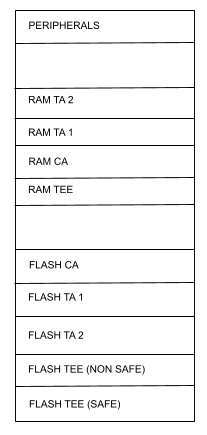
\includegraphics[scale=0.4]{images/memory_map.png}
        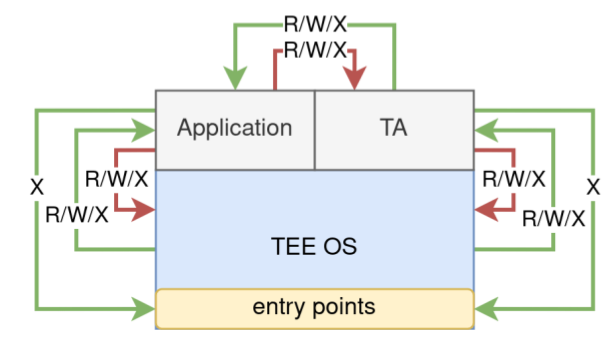
\includegraphics[scale=0.30]{images/acp.png}
	\caption{Simplified memory organization of device running MCU-Fortifier and the access control policy for each component}
	\label{fig:design_mem_map}
\end{figure}

The TEE is stored in two flash memory segments: one accessible (R/W) and executable only by privileged code which contains the core of the Microvisor, while the other accessible and executable by every component containing unprotected code and shared libraries (e.g. C standard library). The Client Application is stored in another section and can be read and executed by unprivileged code. Additionally, privileged code has full access (R/W/X) on it. Regarding the Trusted Application, each of them has a defined section that can be accessed only by itself and the privileged code. Other trusted applications and the untrusted application can not access it.   

The CA RAM is accessible by both privileged and unprivileged code, while similar rules as for the flash memory apply to the RAM sections dedicated to the microvisor and the trusted applications.

\subsection{Enforcing ACP}
After illustrating how memory is organized, in order to enforce the Access Control Policy (ACP) we need to ensure that the CA executes always without privileges and has no way of obtaining them. Should this constraint not be respected the memory isolation would fail since any code running with privileges can access all of the memory and can also modify the configuration of the MPU itself.

As introduced in Section \ref{subsec:exe_mode} any code running in handler mode always executes with privileges, thus we must ensure that the fortified applications always stays in thread mode. In order to execute exception/interrupt handlers without privileges we created a special ``interrupt deprioritization routine'' which activates immediately upon entering handler mode, performing a context switch and returning to thread mode while setting up the execution of the correct exception handler.

Unfortunately executing an application without privileges introduces a series of problems. As previously mentioned system configuration aspects such as interrupts enabling and priorities are stored in the PPB which requires privileged access. 
Since the fortified application must be able to perform these essential configuration steps but cannot access the required memory, the microvisor needs to catch each attempted access and fulfill them in a controlled manner.

Another problem are system instruction. Contrary to PPB accesses, system instructions do not trigger any exception upon being executed without privileges. Instead, their behavior is different sometimes being completely ignored and acting as \verb*|NOP| instruction. To handle these, we created a custom module which is called during the compilation process of the fortified application and performs assembly-level instrumentation in order to highlight for the microvisor the presence of these instruction. This module is what we introduced in Section \ref{sec:intro} as \textit{Instrumenter} and together with the GNU ARM Embedded Toolchain forms what we refer to as \textit{custom toolchain} or \textit{modified toolchain}.

Regarding the enforcement of the strict access rules defined for the memory, the MPU (Memory Protection Unit) was extensively used. In particular, as the number of regions for the MPU of the target device was limited to 8, extensive use of the background region and subregions was made. In particular, when the CA is launched, it does not have access to areas other than its own. As soon as a call to a TA API is made, the MPU regions are reconfigured based on the Trusted Application called to allow access to the specific areas needed. When the API call terminates, the MPU is configured back to its original setup. 

\subsection{Previous Design}
Before discussing the implementation of MCU-Fortifier we want to analyze the design of a previous version of MCU-Fortifier and the reasons why this was quickly abandoned.

Previous design iterations of MCU-Fortifier used a completely software-based approach. The goal was to provide memory isolation to a wider range of devices even those not equipped with an MPU. This design follows an approach similar to S$\mu$V\cite{suv} and $\mu$MSP\cite{msp} dividing the assembly instruction in two groups: \textit{safe} and \textit{unsafe} instructions.
Additionally, unsafe instructions can be further classified as \textit{implicit} or \textit{explicit}.

An instruction is classified as \textit{unsafe implicit} if its execution might result in a violation of the ACP. Unfortunately, this cannot be determined statically at compile time but only at runtime.
The solution is to virtualize all unsafe implicit instructions, which can be done using assembly-level instrumentation in order to replace each instruction with a call to the correct virtual function.

However, this approach is not practical for the ARMv7-M architecture. In fact, ARMv7-M mainly uses only two instructions to access memory: load and store. These instructions are used very frequently throughout the program and almost all occurrences are classified as implicitly unsafe.

This result in the need of virtualizing an extremely large number of instructions resulting in heavy overhead, both in terms of code footprint and CPU time. In our initial implementation following this design, instrumenting applications resulted in a 3-fold increase in binary size.

Considering the limited resources of embedded devices, both in terms of memory and CPU, we decided to abandon this approach in favor of the current MPU-based design.

\newpage
\section{Implementation}
\label{sec:implementation}
In this section we will discuss the implementation, analyzing the different challenges that arose during development and how they were handled.

MCU-Fortifier was initially developed on an STM32WB55 board equipped with a Cortex M4 processor. Although MCU-Fortifier is conceived to work on Cortex M3 devices using a Cortex M4 board for development does not represent a problem. In fact, Cortex M4 devices constitute an evolution of Cortex M3 and as such are capable of running all of their instructions and also additional ones. For this reason, although the development was carried out on Cortex M4 hardware, only features available also on Cortex M3 devices were actually used.

Later in the development a decision was made to switch to a B-L475EIOT01A1 board, equipped with an STM32L475 MCU. This was done in order to have access to a wider range of communication peripherals (mainly 2.4GHz Wi-Fi) which allows to better demonstrate the OTA secure update capabilities that MCU-Fortifier provides. For the rest of the manual every mechanics or features specific of the target board used during development will be explicitly pointed out if necessary.

\subsection{Removing Privileges}
As previously mentioned, in order to enforce the ACP, the fortified application must always be executing without privileges. Code executing on an ARMv7-M architecture can ``obtain'' privileges in two different ways:
\begin{enumerate}
	\item During \textit{Thread Mode} by clearing\footnote{Setting to zero} the \textit{nPRIV} bit of the \textit{CONTROL} register.
	\item By entering \textit{Handler Mode}, which as already explained in Section \ref{subsec:exe_mode} always executes with privileges.
\end{enumerate}

Preventing the application from clearing the nPRIV bit is quite easy. In fact, before the fortified application is executed, the microvisor code sets this bit to one. Once nPRIV has been set, it can only be cleared by code executing with privileges. Therefore, if an application always executes in thread mode there would be no way for it to obtain privileges and change this value once again. In practice this assumption is false because entering handler mode allows the fortified application to obtain privileges. For this reason we created a special \textit{interrupt deprioritization} process which prevents the fortified application from ever handler mode.

\subsection{Interrupt Deprioritization}
\label{subsec:deprio}
Assuming that an application never enter handler mode is unrealistic. In fact, the architecture automatically enters handler mode when servicing interrupts/exception which are a fundamental feature used by almost all applications.

In the ARMv7-M architecture, interrupts are considered as a special type of exceptions. Furthermore each interrupt/exception is paired with its own \textit{handler}, sometimes called ``exception handler'' or ``interrupt service routine''.

The association between each exception and the respective handler are stored in the \textit{vector table} in the form of pointers to functions. During the normal execution of the application when an exception is triggered, the processor looks through the vector table, finds the handler associated with the exception, switches to handler mode and starts executing it. This is done automatically by the architecture without any need for the developer to write custom code. Furthermore the architecture follows the AAPCS (ARM Architecture Procedure Call Standard), therefore the exception handler can be implemented exactly as any ``regular'' function.

For this mechanism to work the processor must know where the vector table is stored, which can be specified through the use of the \textit{Vector Table Offset Register} or \textit{VTOR} in short. Normally, the table is stored at the lowest available address of flash memory, but it can be useful to change its location which, as will be explained later, is exactly what MCU-Fortifier does.

MCU-Fortifier Interrupt Deprioritization is composed of the following 3 routines:
\begin{enumerate}
	\item \textit{Exception Catcher}: catches an exception when it occurs. This function replaces the original exception handler normally called by the exception.
	\item \textit{Exception Simulator}: sets up the context (priority and privileges) in order to execute the original exception handler while being in thread mode.
	\item \textit{Exception Return}: performs a correct return form exception once the original exception handler has been executed.
\end{enumerate}

\subsubsection{Exception Catcher}
Our end-goal is to prevent fortified application code from being executed in handler mode. Additionally, such mode is automatically entered upon triggering an exception. For this reason, MCU-Fortifier replaces all exception handlers in the vector table in order to execute a routine under its own control, this being the \textit{Exception Catcher}.

In the actual implementation, the original vector table of the fortified application is not modified. Instead, the flash memory stores 3 different vector tables at all times:
\begin{itemize}
	\item Vector table 1: stored at the beginning of the microvisor flash memory, contains ``conventional'' exception handlers used by the microvisor during the boot phase (e.g. communication with GPIO, I$^2$C busses, SysTick etc.).
	\item Vector table 2: stored after the previous vector table. This table is mostly filled with \textit{Exception Catcher} entries replacing the conventional handlers. The microvisor sets the VTOR in order to point to this table immediately before beginning the execution of the fortified application.
	\item Vector table 3: stored at the beginning of the fortified user application memory. This is the original vector table of the fortified application. The VTOR never points to this table, instead the \textit{Exception Simulator} access it during its execution in order to recover the original handlers that must be executed without privileges.
\end{itemize}

During the execution of the fortified application each time an exception is triggered, the architecture automatically looks up in vector table 2 (because pointed by VTOR) the handler to execute. This handler will be the \textit{Exception Catcher} routine.

The Exception Catcher then performs the following actions:
\begin{itemize}
	\item Disables interrupts, allowing to execute the rest of the actions in an atomic fashion.
	\item Saves key contextual information of the pre-empted code on the main stack pointer. The ARMv7-M architecture provides two different stack pointers, PSP (Process Stack Pointer) and MSP (Main Stack Pointer). During handler mode MSP is always used. In Thread mode instead, either of the two can be used depending on the value of the \textit{SPSEL} bit the \textit{CONTROL} register.
	
	In particular are saved: all the registers not automatically saved by the architecture, the \textit{EXC\_RETURN} value (indicating which mode and stack the processor should use after exception return) and the priority of the pre-empted code (in the form of the \textit{BASEPRI} value of the special purpose \textit{mask registers}).
	
	This information is necessary in order to correctly resume the execution of the pre-empted code after the original handler has been executed without privileges.
	\item Enables Thread Mode privileges, required for the correct execution of \textit{Exception Simulator}.
	\item Creates an additional ``fake return frame'' on the MSP and performs the exception return. During the exception return, the architecture automatically unpacks this frame which is set-up in order to return the processor to Thread Mode (with MSP in use) and pass the control to \textit{Exception Simulator}.
\end{itemize}

\subsubsection{Exception Simulator}
After the exception return, \textit{Exception Simulator} beings executing (using Thread Mode, with privileges enabled and MPS in use) and performs the following:
\begin{itemize}
	\item Sets the correct execution priority for the handler to be executed. In ARMv7-M, the execution priority governs whether another exception can pre-empt the current instruction stream or not.
	\item Re-enables interrupts.
	\item Removes Thread Mode privileges.
	\item Partially restores the original context (r4-r11) that was manually saved during Exception Catcher.
	\item Performs a branch and link (\verb|BL| instruction) to the original exception handler that must be executed without privileges.
\end{itemize}

At this point, the original exception handler starts begin executed in Thread Mode without privileges while retaining the original execution priority. This way, if an interrupts with higher priority occurs, it will still pre-empt the instruction stream therefore maintaining the original behavior of the ARMv7-M architecture.

As any other function, the last instruction of an exception handler is a return, which normally begins the exception return process. However, since we removed the \textit{EXC\_RETURN} from the link register, the exception return process is not performed and the control is returned to Exception Simulator as wanted.

At this point ideally we would like to re-obtain the privileges and resume the instruction stream originally pre-empted. Unfortunately this is not straight-forward due to two reasons:
\begin{itemize}
	\item As previously mentioned, code running in Thread Mode without privileges cannot change the value of \textit{nPRIV}. The only way to re-gain privileges is to enter Handler Mode and modify \textit{nPRIV} form there.
	\item Performing the stack unwinding process, necessary to resume the instruction stream pre-empted, consists in writing content to 16 registers: r0-r12, LR, PC, xPSR. Unfortunately, the xPSR register (combination of IPSR, APSR and EPSR) cannot be explicitelly written to, in fact the ARMv7-M architecture implements it as WI (Write Ignored).
\end{itemize}

To solve both of these problem the Exception Simulator triggers a HardFault on purpuse in order to enter Handler Mode. A HardFault is a type of exception always enabled which can be easily triggered by performing an unprivileged access to the PPB. From the HardFault hanlder, the control is passed to the \textit{Exception Return} routine.

\subsubsection{Exception Return}
\label{subsubsec:exc_ret}
The Exception Return routine is tasked with restoring the original context and resuming the pre-empted instruction stream.

It begins by performing a check on the PC to evaluate at which point during the execution the HardFault occurred. If the HardFault occurred at the end of the Exception Simulator routine, as expected, than it's treated as an ``exception return request''. Otherwise the HardFault must have been triggered by a different error so the control is returned to the HardFault handler.

If the HardFault was generated as a way to request an exception return, the routine does the following:
\begin{itemize}
	\item Removes the stack frame created on exception entry. This was created due to Exception Simulator triggering the HardFault, of course we have no interested in resuming that execution since we triggered the exception on purpose as a way to properly return to the original instruction stream.
	\item Clear the \textit{CFSR} (Configurable Fault Status Register) which contains information about the fault that was triggered. In our case its content was altered during after Exception Simulator triggered the HardFault.
	\item Unwind the remaining content of the stack stored manually during the Exception Catcher, while also restoring the original execution priority of the pre-empted code.
	\item Perform the exception return using the original frame, created automatically by the architecture during the transition form the originally pre-empted code to the Exception Catcher.
\end{itemize}

As a side note, during the execution of this routine there is no need to manually disable and re-enable interrupts in order to execute it atomically. In fact, when a HardFault is triggered, the corresponding handler executes automatically at the highest possible priority which ensures that our code will not be pre-empted.

\subsubsection{Mask Register and Priority}
System instructions such as \verb|CPS| (Change Processor State) can modify the value of \textit{PRIMASK} and \textit{FAULTMASK}. These are normally used to disable interrupts because they raise the execution priority to a high value (0 or -1 respectively). In the Exception Catcher we set both \textit{PRIMASK} and \textit{FAULTMASK} to 1, but in the Exception Simulator we only consider \textit{PRIMASK}. This is because \textit{FAULTMASK} is automatically cleared by the architecture during a return from exception. Furthermore, Exception Simulator can keep \textit{PRIMASK} set as a way to raise the execution priority to 0, which is required if the original exception handler was configured with that priority value.

\subsubsection{Limitations}
\label{subsubsec:limitations}
Due to the stack manipulation that occurs both in Exception Catcher and Exception Simulator, the stack differs from what would normally happen in a regular execution without interrupt deprioritization. For this reason, the fortified application handlers cannot rely on contextual information stored on the stack (e.g. by pushing data onto the stack before triggering the exception on purpose). This assumption is reasonable. In fact, interrupt handlers generally behave independently of the address on which the interrupt was triggered and tend to access global data structures using static references, which are stored intermixed with the assembly code. \textit{SVCall} exceptions, however, violate this assumption and require the additional measures described in Section \ref{subsubsec:svc}.

\subsubsection{Virtual IPSR}
\label{subsubsec:virtual_IPSR}
Some OSes commonly used on embedded devices (e.g. Mbed OS), explicitly read the IPSR (Interrupt Program Status Register) to check whether an exception is being processed and branch to different code. Of course MCU-Fortifier must be transperent in this regard, ensuring that the behavior of the fortified application is the same as the non-fortified one.

Unfortunately, as previously described, the interrupt deprioritization routine executes handlers in thread mode (meaning that during their execution IPSR is set to 0). For this reason, if the check is performed during an interrupt handler, the result would differ when using the fortified application.

To solve this problem we implemented a \textit{Virtual IPSR}, which is a global variable stored in the microvisor reserved RAM. The virtual IPSR reflects what the real value of the IPSR should be, meaning that during the execution of the deprioritized handlers it will still contain the correct number of the exception being handled even though the code is running in thread mode.

The virtual IPSR is manipulated in 3 different locations:
\begin{enumerate}
	\item During the Exception Catcher, the current value of the virtual IPSR is saved on the stack, in order to be restored when resuming the execution of the pre-empted code.
	\item During Exception Simulator, the value of the virtual IPSR is set to the correct exception that will be handled in thread mode.
	\item During Exception Return, the value of the virtual IPSR saved on the stack is restored.
\end{enumerate}

The implementation of the virtual IPSR is particularly straight forward. Every access to the ``real'' IPSR must be done using the system instruction \verb|MRS| and \verb|MSR| (respectively for read and write access). As we will explain in Section \ref{subsubsec:system_instructions} these instruction must be virtualized because their behavior changes based on whether they are executed with privileges or not. During this virtualization, we can simply redirect every read/write access of the real IPSR to our virtual IPSR.

\subsubsection{Integrity checks on exception return}
The ARMv7-M architecture performs automatically different integrity checks during exception return. In particular, when returning from an exception to thread mode, the architecture checks that no other exception (beyond the returning one) are active. This would indicate a mismatch in the number of exception return, since when returning form an active exception to another one handler mode should be maintained.

Unfortunately, this checks directly affects our interrupt deprioritization routine. We will use an example to illustrate why this integrity check is problematic:
\begin{itemize}
	\item Suppose that there are two interrupt A and B, with B having higher priority than A (therefore able to pre-empt its execution).
	\item Interrupt A is triggered and the Exception Catcher routine for interrupt A starts being executed (interrupt A becomes active).
	\item Before Exception Catcher disables interrupts (with the \verb|CPS| instruction), interrupt B is triggered and pre-empts the execution of interrupt A (both B and A are now active). The Exception Catcher routine for interrupt B starts being executed).
	\item The Exception Catcher routine for interrupt B completes and an exception return is performed in order to pass control to Exception Simulator.
	\item This will result in the integrity check failing because B is trying to return in thread mode (in order to execute Exception Simulator) but A is still active.
\end{itemize}

Fortunately for us, this is the only integrity check relevant for our implementation. Additionally, this check can be disabled by setting the \textit{NONBASETHRDENA} bit of the \textit{CCR} (Control and Configuration Register). This operation is done at boot by the microvisor, before switching vector table and passing control to the fortified application.

\subsection{Issues of Unprivileged Execution}
Now that we have shown how to obtain the fortified application running always without privileges, we need to tackle the different problems that this practice creates. Mainly the problems are:
\begin{enumerate}
	\item PPB accesses: unprivileged access to the Private Peripheral Bus trigger an HardFault.
	\item System instructions: ARMv7-M system instructions behave differently depending whether executed with privileges or not.
	\item SVCall exception: SVCall exception needs to recover SVC number by accessing stack and recovering PC value during exception entry. This cannot be done due to the limitations highlighted in Section \ref{subsubsec:limitations}.
\end{enumerate}

\subsubsection{PPB Access}
\label{subsubsec:PPB_access}
Accessing the PPB is fundamental for every application. In fact, this region of memory stores global system configuration, such as the list of enabled interrupt and their priority, therefore we need a way to provide access to unprivileged applications.
Simultaneously, we cannot allow access to every register in the PPB. For example, the fortified application should not be able to modify the configuration of the MPU, neither it should be able to access the VTOR.

Granting access to these registers would allow the fortified application to circumvent the ACP, either by removing MPU restrictions and allowing access to the whole system memory, or by removing the interrupt catching sequence and allowing it to enter handler mode uncontrolled. For these reasons we need to control PPB accesses on a one-by-one basis.

To do this, a special ``PPB Access Recovery'' routine was created which exploits the fact that an unprivileged access to the PPB triggers an HardFault\footnote{To be precise a BusFault is triggered, if such exception is disabled the ARMv7-M architecture escalates the fault to a HardFault}. The PPB recovery routine is called inside the HardFault handler, after having checked that the HardFault was not triggered by an exception return request (Section \ref{subsubsec:exc_ret}). It performs the following:
\begin{enumerate}
	\item Checks the PC address at the time of the HardFault and reads the instruction which caused it.
	\item Checks whether the instruction is a variation of load or store (considering single byte, half word and word accesses).
	\item Using a complex pattern matching sequence, decomposes the operands of the instructions (accessed address, registers that would be stored/loaded).
	\item Checks the permission that the fortified application has on the accessed address.
	\item Depending on the permissions, carries out the operation for the application by ``simulating'' it and advances the program counter.
	\item Clears the CFSR and resumes the execution of the pre-empted code.
\end{enumerate}

\paragraph{Permissions}
In the context of PPB access recovery, permissions refer to the following:
\begin{itemize}
	\item Not a PPB access: the address the fortified application is trying to access is not part of the PPB. In this case the functions returns. The HardFault was not caused by an unprivileged PPB access, the HardFault handler will regain control and process it.
	\item Read, Write: the address accessed is indeed part of the PPB. The fortified application has both read and write access on it, the instruction should be executed. For example, this is the case for all NVIC configuration registers used for enabling, disabling and setting interrupt priorities.
	\item Read Only, Write Ignored: the address accessed is part of the PPB. The fortified application can read the value of such registers but should not be able to write to them. More specifically, during a write attempt, the program counter is advanced but the write operation has no effect, therefore continuing the execution of the fortified application while effectively skipping the store instruction. For example, this is the case for registers concerning MPU configuration and VTOR.
\end{itemize}

\paragraph{Instruction Simulation}
By ``simulation'' we refer to the way the problematic instruction is executed by the microvisor. In particular, the execution is performed by creating a \textit{virtual function}\footnote{A temporary function stored in volatile memory} in a specific region of RAM. In this virtual function there are only two instructions: the problematic load/store instruction, followed by a return. At most this only requires 3 half word of memory (48 bits): one word for the problematic instruction (which could be either 16 or 32 bits depending on the encoding), one half word for the return instruction (\verb|BX LR|, always encoded using 16 bits).

This approach was chosen because it massively simplifies the implementation. In fact, the alternative would be to dissect every instruction down to every single bit of their encoding (e.g. evaluate whether offset, pre-indexed or post-indexed addressing mode is being used, checking whether the instruction updates the condition flags in the \textit{APSR}, and many other aspects) and the effect manually. Naturally, such an approach would massively increase the complexity and footprint of the code. Instead our ``simulation'' approach is much simpler as it does not need to consider all of these aspects.

Unfortunately, our approach has a limitation: not every single instruction can be executed in this way. 
In order for the simulation to be accurate, we must restore the execution context present during the original instruction. Additionally, this context will be updated with new values generated during the simulation and will be used to resume the original instruction stream.

In practice we can do this only for the general purpose register r0-r12 and the \textit{APSR}. Which leaves us with altered values (compared to the original instruction execution) for registers SP, LR and PC. SP register is altered by the stacking operations performed on exception entry and our additional function calls. Altering LR is necessary in order to perform the return from the virtual function to its caller. Finally, PC will differ because we are executing the virtual instruction (stored in RAM) instead of the original one (stored in its original location in flash memory).

Fortunately, none of these registers are normally used as operands in the instructions concerning us. Intuitively, we can understand how none of these registers (SP, LR and PC) would sensibly be used as source or destination. No real-world code would find use into reading content from the PPB and storing it in one of these register, nor it would be useful to store the content of these registers into any part of the PPB. Additionally these registers are also never used to address the PPB. PC and SP-relative addressing are indeed used in the ARMv7-M architecture, but these operation are useful only to access memory areas near the SP (to retrieve data on the stack) or near the PC (to retrieve data intermixed within the code). Obviously in no real-world application SP will point anywhere near PPB areas, instead it will point to volatile memory. Neither will PC, since the PPB and regions of memory in its proximity are not executable

Nevertheless, even if such corner cases were to happen our implementation is capable of detecting them and prevent violation of the ACPs.

\subsubsection{System Instructions}
\label{subsubsec:system_instructions}
Although barely mentioned in the manual, the ARMv7-M system instructions behave differently depending on the level of privilege during their execution. In particular the architecture provides 3 system instructions:
\begin{itemize}
	\item \verb|CPS| (Change Processor State), is used to change the value of \textit{PRIMASK} and \textit{FAULTMASK} in the mask register. Any unprivileged execution of this instruction has no effect on the masks.
	\item \verb|MRS| (Move to Register from Special register), allows to read the value of different registers (xPSR, MSP, PSP and mask register). When executed without privileges any attempt to read IPSR, MSP, PSP or mask register will return zero.
	\item \verb|MSR| (Move to Special register from Register), allows to write values to special registers (APSR, MSP, PSP, mask register and CONTROL register). When executed without privileges, any attempted write to MSP, PSP, mask register and CONTROL register will be ignored.
\end{itemize}

Considering that our goal is to make the fortified application run without privileges while keeping its original behavior, we need a way of executing these instructions as if they were executed with privileges, while also being transparent to the fortified application. Unfortunately, unlike PPB accesses, the unprivileged execution of these instruction does not cause any ``observable'' exception.

For these reason it was necessary to implement custom assembly-level instrumentation, which allows the microvisor to detect any attempt of the fortified application to execute system instructions. After these have been detected, a mechanisms analogue to the PPB access recovery is triggered in order to carefully control and carry out the accesses on a one-by-one basis.

\paragraph{Instrumentation}
The assembly-level instrumentation is implemented through the use of a Python 3 script.

The purpose of this script is to insert an \verb|SVC 0| instruction immediately before every system instruction. In this way, an \textit{SVCall} exception is triggered before the execution of every system instruction, rendering them  observable.

Additionally, the instrumentation decomposes every \verb|IT| conditional instruction whose block covers system instructions. This is performed due to complexities that arises when dealing with conditional execution through \verb|IT|\footnote{See \textit{ITSTATE} in ARMv7-M Manual\cite{armv7m}} and the correct restoration of context during a return from exception.

The decomposition consists in removing the whole \verb|IT| instruction and inserting, before each of the instructions covered by \verb|IT|, a conditional branch. The purpose of the branch is to skip the instruction when the necessary conditions for execution are not met. This provides the same behavior of the originally replaced instruction while slightly increasing the size of the code.

\paragraph{SVCall Exception}
At runtime, the \verb|SVC| instruction inserted triggers an exception: \textit{SVCall}. This exception is then handled by the microvisor \textit{SVCall} exception handler (sometimes called \textit{SVC Handler}), which recovers the execution of system instruction similarly to what explained in Section \ref{subsubsec:PPB_access} for PPB accesses.

In particular the following operations are performed:
\begin{enumerate}
	\item The value of the program counter prior to exception entry is recovered. And the instruction following the one that triggered the exception (\verb|SVC 0|, inserted by our instrumentation) is recovered.
	\item If such instruction is one of \verb|CPS|, \verb|MRS| or \verb|MSR|, a ``simulation'' process analogue to the one described in Section \ref{subsubsec:PPB_access} is performed, using a virtual function containing a copy of the problematic instruction (in this case a system instruction instead of a load/store).
	\item Otherwise, an ``original'' (not inserted by our instrumentation) \verb|SVC| instruction was encountered. The microvisor manually launches the interrupt deprioritization process by calling the Exception Catcher routine.
\end{enumerate}

Additionally, during the simulation of system instruction the behavior of \verb|MRS| and \verb|MSR| is altered on purpose in the following way:
\begin{itemize}
	\item In \verb|MRS|, any read targeting the \textit{IPSR} is redirected to our virtual IPSR. This renders the interrupt deprioritization process transparent to the fortified application as discussed in Section \ref{subsubsec:virtual_IPSR}.
	\item In \verb|MSR|, any attempt to write the \textit{nPRIV} bit of the \textit{CONTROL} register is ignored\footnote{Done automatically by the architecture when MSR is executed in thread mode, however simulation occurs in handler mode so we need to manually alter its behavior}. This prevents the fortified application from re-gaining privileges in thread mode execution.
\end{itemize}

\subsubsection{SVC Instruction and SVCall Exception}
\label{subsubsec:svc}
The \verb|SVC| (SuperVisor Call) instruction, is provided by the ARMv7-M architecture in order to facilitate the separation between an application and a possible operative system running on the device. The \verb|SVC| encodings allows to specify an 8-bit integer (sometimes called \textit{SVC number}) which can be used as a way to pass an argument to the \textit{SVCall} handler.

\paragraph{TEE SVC Handler}

The Trusted Execution Environment (TEE) heavily relies on the Supervisor Call (SVC) mechanism to simulate privileged instructions, change the context, privileges level, and call the appropriate GP API. In particular, the SVC Handler of the Microvisor can be called and executed for the following reasons. 
\begin{itemize}
    \item Simulation of a system instruction (the SVC was called due to the CA code instrumentation): in that case, the instruction is simulated without priviledges and the exception return procedure is performed; 
    \item Call of a TEE Client API: the SVC was used by the client application to perform a Global Platform  Client API call (SVC number is in the range 0-4). In that case, the API call is used to invoke the requested TA and the exception return is performed;
    \item Call of a TEE Core API: the SVC was called by a trusted application to perform a TEE Core API call (SVC number is in the range 5-50). In that case, the API call is performed and the execution is returned to the trusted application;
    \item CA SVC call: the original SVC\_Handler is needed and the control should be passed to the appropriate deprioritized handler.
\end{itemize}

\paragraph{CA SVC Handler}
The way \textit{SVCall} handler of the CA is supposed to recover this argument is the following:
\begin{itemize}
	\item Read the frame created during exception entry and retrieve the pre-entry PC value.
	\item Read the instruction stored at the address specified by PC (the encoded \verb|SVC| instruction).
	\item Extract the 8-bin integer by reading the least significant byte of the instruction.
\end{itemize}

Unfortunately, this goes directly against the limitation (discussed in Section \ref{subsubsec:limitations}) which prevents deprioritiezed handlers from using the stack values stored by the architecture during exception entry. Due to the stack being manipulated by our interrupt deprioritization routines, \textit{SVCall} handler does not find the value of the PC in the expected location.

This is an instance where source code modification to the fortified applications is required, albeit being minimal. In fact, the microvisor \textit{SVCall} is designed to recover the SVC number (during the microvisor own \textit{SVCall} handler) and pass it to the deprioritized handler (through \textit{Exception Catcher} and \textit{Exception Simulation} routines) as the first argument using register \verb|r0|.
For this reason, the source code modifications are relatively simple, and in particular, if the \textit{SVCall} is written in C, it suffices to:
\begin{enumerate}
	\item Change the signature of \textit{SVCall} in order to expect an 8-bit unsinged integer as argument (e.g. \verb|void SVCall(uint8_t SVCnum)|).
	\item Remove from \textit{SVCall} the source code originally used to retrieve the SVC number.
\end{enumerate}

\subsection{Memory Protection Unit}
\label{subsec:MPU}
As previosly discussed, the Memory Protection Unit (MPU) plays a fundamental role and is used, in combination with the interrupt deprioritrization routines, to enforce the ACP.

\subsubsection{Using the MPU}
\label{subsubsec:using_mpu}
Before we discuss the default configuration of the MPU provided by MCU-Fortifier, we need to briefly introduce how the MPU works. The MPU allows us to divide the addressable memory space in different sections called \textit{MPU regions}. Each of these region is associated with a set of attributes that specify:
\begin{itemize}
	\item \textit{Region Enable}: whether the region is currently enabled or not.
	\item \textit{Region Number}: numeric index of a region. Higher numbered regions have priority over lower numbered ones.
	\item \textit{Size}: size of the region. Must be defined as a power of two (e.g. 512, 1024, 2048 bytes).
	\item \textit{Base Address}: starting address of the region. Must be naturally aligned based on the region size (e.g. a 2048 bytes sized region must also be 2048 bytes aligned).
	\item \textit{Access Permissions}: read and write permissions. Can be specified separately for privileged and unprivileged code, with the constraint that privileged code permissions are a super set of unprivileged code ones.
	\item \textit{Execution}: whether the region can be executed as code. A pre-requisite for execution is the read access, needed in order to fetch the instructions before execution.
	\item \textit{Sub Region Enable}: allows further sub-divide the region into smaller chunks which can be enabled or disabled individually. Each chunk has inherits the permission from the base region.
	\item \textit{Type Ext (Tex)}, \textit{Sharable}, \textit{Cachable}, \textit{Bufferable}: different combinations of these parameters are set depending on the memory type and properties. For example, ``strongly ordered shared memory'' can be obtained by setting the parameters to respectively: \verb|0 1 0 0|. For more information, consult the ARMv7-M Architecture Manual\cite{armv7m} and the STMicroelectronics AN4838-Application Note\cite{an4838}.
\end{itemize}

When a memory access is performed, the MPU matches the requested address against the different enabled regions. If there is a single matching, the configuration of the region is checked (including if the address match the subregion of that region allocated for that application) in order to evaluate whether the access should be allowed or not. Additionally the regions can be overlapping, meaning that multiple regions might match with a single access. In this case, the rules of the region with highest \textit{region number} are applied.
Accesses that do not match any memory regions trigger a \textit{MemManage} exception.

Setting the \textit{PRIVDEFENA} bit of the \textit{MPU\_CTRL} register allows non-matching accesses and adresses belonging to disabled subregions to use the default memory map specified in the ARMv7-M Architecture Manual\cite{armv7m}. However, this only applies to accesses performed by privileged code. Unprivileged code is not allowed to use the default memory map when the access does not match any region.

Finally, any access to the Private Peripheral Bus (PPB) always uses the default memory map, regardless of how the MPU is configured. Meaning that the MPU is restricted on how it can change memory attributes of the system address space.

\subsubsection{MCU-Fortifier Memory Map}
\label{subsubsec:memory_map}
Before we outline the configuration of the different MPU regions, let's begin by examining MCU-Fortifier memory map for our STM32L475 MCU, detailed in Listing \ref{lst:memory_map}.

\begin{lstlisting}[caption={MCU-Fortifier memory map linker script (memory\_map.ld)},captionpos=b,label=lst:memory_map]
MEMORY
{
FLASH_BOOT (rx)        	   : ORIGIN = 0x08000000, LENGTH = 0x20000  
FLASH_TA1 (rx)             : ORIGIN = 0x08020000, LENGTH = 0x3C000  
FLASH_SECURE_TA1(rw)       : ORIGIN = 0x0805C000, LENGTH = 0x4000  
FLASH_TA2 (rx)             : ORIGIN = 0x08060000, LENGTH = 0x3C000  
FLASH_SECURE_TA2(rw)       : ORIGIN = 0x0809C000, LENGTH = 0x4000    
FLASH (rx)                 : ORIGIN = 0x080A0000, LENGTH = 0x58000   
FLASH_BOOT_NOPRI (rx)      : ORIGIN = 0x080F8000, LENGTH = 0x8000   
RAM_BOOT (xrw)             : ORIGIN = 0x10000000, LENGTH = 0x20 	
RAM (rw)             	   : ORIGIN = 0x10000020, LENGTH = 0x7FE0   
RAM_TA1 (xrw)       	   : ORIGIN = 0x20000000, LENGTH = 0xC000   
RAM_TA2 (xrw)              : ORIGIN = 0x2000C000, LENGTH = 0xC000    
}
\end{lstlisting}

As we can see there are 11 different memory regions:
\begin{itemize}
	\item \verb|FLASH| and \verb|RAM| are the regions which should be accessible to the fortified application.
	
	In particular \verb|RAM| is one of RAM banks available on the board and the fortified application must have read and write access to it, but no execution permission in order to prevent possible self-writing code or remote code injection attacks.
	
	On the other hand, \verb|FLASH| is the region of flash memory where the fortified application is stored. As such, the fortified application should be able to read and execute instructions from this region. Additionally, it should not be able to write to this region, in order to prevent remote code injection and also to protect the integrity of the code.
	
	The microvisor and the TAs, on the other hand, has full access over these regions. In particular, the TAs have access due to the current implementation of shared memory. 
	
	\item \verb|RAM_BOOT| is the region of RAM reserved purely for microvisor usage. It contains the value of the Virtual IPSR (Section \ref{subsubsec:virtual_IPSR}) and the memory used for instruction simulation (Section \ref{subsubsec:PPB_access} and \ref{subsubsec:system_instructions}). The fortified application and the trusted applications should not be able to access this region.
	
	\item \verb|FLASH_BOOT| is the region of flash memory where the microvisor is stored. This region should be accessible in read,write and execute modes only by the microvisor. The fortified application and the trusted applications should not be able to access it.
	
	\item \verb|FLASH_BOOT_NOPRI| this region contains microvisor code that must be executed without priority. An example is the code used to bootstrap the execution of the fortified application after the thread mode privileges have been disabled by the microvisor, the shared libraries and the entry points for the Global Platform Core API. This region should be readable and executable by unprivileged software. As a consequence, fortified applications and trusted applications are also able to access this region meaning that sensitive data should never be stored here.

    \item \verb|FLASH_TAx|, \verb|FLASH_SECURE_TAx| and \verb|RAM_TAx| are the regions which should be accessible to the trusted application number . 

    In particular \verb|RAM_TAx| is (part of) the other RAM bank available on the board and the trusted application ''X'' must have read and write access to it, but no execution permission in order to prevent possible self-writing code or remote code injection attacks. The physical bank is shared with the \verb|RAM_TAy| using subregions and activating only the part of the RAM used by the current TA. To recap, the TA ''Y'' does not have access neither for read, write or execute on this section, as well as the fortified application. The microvisor can perform every operation on this memory area.  
	
	On the other hand, \verb|FLASH_TAx| and \verb|FLASH_SECURE_TAx|are the region of flash memory where the trusted application ''X'' is stored and store its secure data. As such, only the trusted application x should be able to read and execute instructions from the flash region and read and store data in the flash secure one. As for the RAM, the TAy and the fortified application have no permission on that area, while the microvisor has them all. 
\end{itemize}

The ARMv7-M architecture does not provide a standard number of MPU regions supported by the processor. Instead, each manufacturer implementation might provide a different number. In our case, the STM32L475 processor is capable of providing support for up to 8 MPU regions (numbered from 0 to 7). Each region can be further divided into 8 sub-regions of the same size (numbered from 1 to 8), that can be activated or deactivated based on the needs. 

Although we have provided a list of different memory ares, these are not the only areas that we need to consider using the MPU. In fact, every memory address performed by the fortified application must be covered by an MPU region (otherwise a MemManage exception would be generated), this includes also memory areas such as: memory mapped peripherals, system memory, option bytes and OTP (One Time Programmable) memory normally available on STM32 boards.

In general, the MPU configuration we provide is specific to the STM32L475 MCU and based on the memory map described in its reference manual\cite{rm0351}.
Additionally, we have tested this configuration with multiple fortified applications and we have observed that all accesses are covered by the different regions. Nevertheless, our testing is not exhaustive by any mean and special purpose applications might access memory regions not covered by any MPU region.

\subsubsection{MPU Configuration}
\label{mpu-config}
Since some regions of memory previously outlined are not sized as powers of two and are neither naturally aligned, we cannot simply map them one-by-one to MPU regions. Instead, we use a set of MPU regions to grant permissions to the unprivileged code in a coarse-grained fashion. Then, we use a second set of MPU regions, overlapping with the first set, in order to restrict access to the memory areas that should be accessible only by privileged code. To ensure that the fine-grained restrictions applied by the second set have priority over the first set, we use regions with a higher MPU number.

In our default configuration, used during the startup of the system and when the system normally executes the fortified application (not the trusted ones) we identified the following 8 MPU regions, with MPU numbers ranging from 0 to 7:
\begin{enumerate}
	\setcounter{enumi}{-1}
	\item Flash memory: region covering the entirety of the flash memory, with a base address \verb|0x08000000| and size of \verb|0x100000| (1 MB). This area contains, respectively, the code and data for the CA, both TAs, the TEE and TEE area accessible without priority and it is readable and writable by privileged code, but only readable by unprivileged. Execution allowed. To restrict the possibility of unstrusted application on this huge are, the Region 1 is used to make the Microvisor reserved flash unaccessibile and subregions to make the flash for TAs inaccessible. This requires to have dedicated sections for the TAs that are aligned with the size of one subregions, each of size \verb|0x20000| (128KB), or a multiple of that. During this phase, the subregions assigned to the TA1 and TA2, namely the number 2,3,4 and 5 should be disable in order to prevent access, even in read only mode, to untrusted applications. 
	\item Microvisor reserved flash: region covering the flash memory reserved for microvisor usage (excluding \verb|FLASH_BOOT_NOPRI|). With base address \verb|0x08000000| and size \verb|0x20000| (128 KB). Readable and writable by privileged code, not accessible by unprivileged. Execution allowed. This region overlap the previous one and restricts CA and TAs form accessing microvisor reserved flash.
	\item RAM for TAs: region covering the entirety of bank 1 RAM. With base address \verb|0x20000000| and a nominal size of \verb|0x20000| (128 KB). The real allocatable size of \verb|0x18000| (96 KB) would suffice, but is not a power of two so we select the smallest immediately greater power of two. In this configuration the MPU region ``overflows'' the RAM but it does not represent a problem since the following memory is reserved\footnote{As indicated by the MCU reference manual\cite{rm0351}} and should never be accessed anyway. Readable and writable by privileged code only during the execution of CA. Execution not allowed.
    \item RAM for CA: region covering the entirety of bank 2 RAM, with a base address \verb|0x10000000| and a size of \verb|0x8000| (32 KB). Readable and writable by both privileged and unprivileged code. Execution not allowed.
	\item Microvisor RAM: region covering the RAM reserved for microvisor usage. With base address \verb|0x10000000| and size \verb|0x20| (32 B). It partially overlaps the RAM region for the CA and imposes stricter privileges, thus the section is readable and writable by privileged code, not accessible by unprivileged. Execution allowed, needed for the execution of the virtual function explained in Sections \ref{subsubsec:PPB_access} and \ref{subsubsec:system_instructions}.
	\item Peripheral address space: memory space used to access memory mapped peripherals. With base address \verb|0x40000000| and size \verb|0x40000000| (1 GB). Readable and writable by both privileged and unprivileged code. Execution not allowed. Configured as ``device'' memory.
	\item Peripheral address space (continuation): configured exactly as the previous entry but with base address \verb|0x80000000|. Unfortunately, using a single MPU region with size of 2 GB caused problems, therefore both region 4 and 5 are necessary.
	\item System memory, option bytes, OTP area: region covering multiple features of STM boards normally used by applications. With base address \verb|0x1fff0000| and size \verb|0x10000| (64 KB). Readable and writable by privileged code, ready-only by unprivileged. Execution not allowed.
\end{enumerate}

With these regions, we can obtain the properties highlighted in Section \ref{subsubsec:memory_map}.

We can notice how the \verb|FLASH_BOOT_NOPRI| does not require a region on its own. In fact, MPU region 0 already covers this memory section and allows the execution of unprivileged code.

The attributes TEX, Sharable, Cachable and Bufferable for all the regions discussed are set accordingly to the specification of the ARMv7-M manual for the system address map\cite{armv7m}. A comprehensive explanation for these attributes can be found in the STMicroelectronics AN4838-Application Note\cite{an4838}.

When a TEE Client API is called, triggering the execution of a Trusted Application (TA), the MPU must be reconfigured to ensure the correct access control policy is enforced for the target TA (e.g., TA1 or TA2). The key changes to the MPU regions include:
\begin{enumerate}
    \setcounter{enumi}{-1}
    \item Flash memory: the subregions associated with the target TA should be enabled (namely 2 and 3 for TA1 and 4 and 5 for TA2), while those corresponding to other TAs should remain disabled. The other subregions (associated with the TEE or with CA) are left unchanged.
    \item Microvisor reserved flash: no changes.
    \item RAM for TAs: the region is divided into subregions of 16KB (considering a nominal size of 128KB for the whole region), thus only the first 6 subregions can be used (given the physical size of 96KB). For this reason the the first three subregions are dedicated to TA1 (namely 1,2 and 3) while the following three (4, 5 and 6) are dedicated to TA2. The subregions associated with the target TA should be enabled, while those corresponding to other TAs should remain disabled. The last two subregions can not be used. 
    \item RAM for CA: no changes, as this regions contains also the shared memory data between CA and TA.
    \item Microvisor RAM: no changes.
    \item Peripheral address space: no changes.
    \item Peripheral address space (continuation): no changes.
    \item System memory, option bytes, OTP area: no changes.
\end{enumerate}

Once the API call is completed, the MPU is restored to its original configuration, allowing the CA to resume normal execution.

For a TEE Core API call originating from a Trusted Application, no MPU reconfiguration is required, as Core APIs are services provided by the TEE and execute directly with the necessary privileges.

\subsection{Permanent Storage}
\label{subsec:permanent_storage}
When using MCU-Fortifier, the microvisor has a need for an area of memory that maintains its content through a board reset. This area is called ``permanent storage'' and is used for storing error logs, among other information, before the device is restarted. Additionally, after these error logs have been reported to an update server, they are wiped from memory.

Given such requirement, the best candidate for this area is flash memory. Unfortunately, using flash memory to store information in such way (logging data and then deleting it successively) is heavily dependent on the flash controller, therefore the device manufacturer.

In our specific case, with the B-L475EIOT01A1 board, the STM flash controller allows in-application programming of the flash albeit subjected to some restrictions. In particular:
\begin{enumerate}
	\item Programming and erasing flash memory is done by accessing the flash controller peripheral.
	\item Write access to flash memory are carried out using double words (writing 64 bits at the time).
	\item Only ``empty'' flash memory can be programmed, attempting to program any non-empty flash memory results in an error. A word of flash memory is considered empty when it stores the value \verb|0xffffffff|.
	\item Flash memory can be erased in mass (completely erasing both banks of memory available on the device), or on a page-by-page basis.
\end{enumerate}

Due to restriction 3 and 4, although we might only need a few bytes to store the information needed, we must reserve an entire page of flash memory. The B-L475EIOT01A1 board is equipped with 1 MB of flash memory split in 2 banks. Each bank contains 256 pages of 2 KB. This means that our permanent storage will be at least 2 KB (2048 bytes) in size.

In the current implementation a single page of 2 KB is more than sufficient to store:
\begin{itemize}
\item MCU-Fortifier Activation Code (32 bytes).
\item Fortified application size (4 bytes).
\item Error ID (4 bytes).
\item Error Data (variable).
\end{itemize}

Each of these fields and their purpose will be described in future sections of this document.

\subsection{TEE Client API}

A TEE Client API is invoked by the Client Application when it needs to use a service provided by either a TA or the TEE. To comply with the GlobalPlatform standard, each TA must implement the following required TEE Client APIs to allow the communication with the Client Application.

\begin{itemize}
    \item Create an entry point for the CA: \textit{TEE\_Result TA\_CreateEntryPoint(void);}
    \item  Open a session to invoke the functionalities of the TA:\\ \textit{TEE\_Result TA\_OpenSessionEntryPoint(uint32\_t param\_types, TEE\_Param params[4], void **sessionContext);}
    \item Execute a command inside the TA:\\ \textit{TEE\_Result TA\_InvokeCommandEntryPoint(void* sessionContext, uint32\_t commandID, uint32\_t paramTypes, TEE\_Param params[4]);}
    \item Close the current session:\\ \textit{void TA\_CloseSessionEntryPoint(void* sessionContext);}
    \item Destroy the entry point for the CA: \textit{void TA\_DestroyEntryPoint(void);}
\end{itemize}

When one of these Client APIs is called using the corresponding function on the CA side (namely \textit{TEEC\_InitializeContext}, \textit{TEEC\_OpenSession}, \textit{TEEC\_InvokeCommand}, \textit{TEEC\_CloseSession} and \textit{TEEC\_FinalizeContext}, several steps must be performed to ensure the successful execution of the TA. 

The CA functions use an \textit{SVC Call} with a number in the range of 0 to 4 to transfer control to the TEE. Additionally, a shared memory data structure, stored in the CA memory area, is used to pass parameters. Specifically, the address of this data structure is stored in register R4 (after saving its original context) and is later retrieved by the appropriate function once the SVC handler is invoked. In the case of a command execution request, the command ID is stored in another register, R5, and recovered in the same manner. All the logic for this process is encapsulated in the library files (\textit{tee\_client\_api.c}, \textit{tee\_client\_api.h} and \textit{tee\_common.h}) which should be included in each CA. After the \textit{SVC Call} invocation, various steps take place inside the Microvisor.

\begin{enumerate}
    \item The SVC handler intercepts the request, recognizes that a Client API call was made, saves the context, and creates a fake return frame.
    \item The Microvisor exits the SVC handler and the corresponding handler mode (still maintaining the privileges), passing control to the \textit{call\_TA} function. This function is responsible for:
    \begin{enumerate}
        \item Transforming the parameters from the CA format to the TA format.
        \item Identifying which TA is being requested by the CA.
        \item Reconfiguring the MPU to run the targeted TA, as described in~\autoref{mpu-config}.
        \item Calling the correct entry point based on the TA number and the SVC number.
        \item Adjusting the stack pointer, as TAs use the Process Stack Pointer (PSP) during execution, while the CA always uses the Main Stack Pointer (MSP).
    \end{enumerate}
    \item The API call is executed, and the TA code runs without privileges.
    \item The output parameters of the TA are copied back and saved. 
    \item The Microvisor regains privileges by simulating a HardFault exception and verifying the source of the error (if it is known, the exception was intentionally triggered).
    \item The exception return is executed, and the MPU is reconfigured to its original state, allowing the CA to resume execution.
    \item The control returns to the original point where the API was called and the context before the SVC is restored.
\end{enumerate}

Note that TAs have standard entry point names, as each TA should offer the same API to communicate with the CA. Since both TAs are compiled alongside the TEE, this poses a problem: multiple instances of a function with the same name would cause a linking error. To address this, the functions in \textit{call\_TA} are defined as \textit{entryPointName\_TaNum}, where TaNum is either 1 or 2, referring to the respective TA. However, within each TA's source code, functions can still be referenced without the suffix. This is achieved by employing the Makefile, which is configured to replace function names in each TA's source code. Specifically, for TA1, the function TA\_CreateEntryPoint is replaced with TA\_CreateEntryPoint1, while for TA2, it is replaced with TA\_CreateEntryPoint2. This renaming applies to all five TEE Client API functions inside a TA. 

\subsection{TEE Core API}

The TEE core API are entry points for basic security services offered by the TEE that can be used only by Trusted Applications (TAs). CA can not use directly TEE Core API, and controls are enforced to prevent this. 

The core APIs exposed by the TEE are divided into different categories, based on their scope. The main ones are the following.

\begin{itemize}
    \item Operation Management functions (e.g., AllocateOperation, FreeOperation, SetOperationKey);
    \item Object Management and Secure Storage functions: operations on transient objects (AllocateTransientObject, FreeTransientObject, PopulateTransientObject, InitRefAttribute, InitValueAttribute, etc.) and on persistent objects (CreatePersistentObject, OpenPersistentObject, CloseAndDeletePersistentObject1, ReadObjectData and WriteObjectData);
    \item Memory Management functions (e.g., Malloc, Free, MemMove);
    \item Random Value generation and Key Generation functions (e.g., GenerateKey and GenerateRandom);
    \item BigInt Functions (e.g., BigIntConvertToS32, BigIntMod, BigIntConvertFromOctetString);
    \item Symmetric Cipher Functions (e.g., CipherInit, CipherUpdate, CipherDoFinal);
    \item MAC functions (e.g., MACInit, MACUpdate, MACComputeFinal);
    \item Message Digest Functions (e.g., DigestUpdate, DigestDoFinal, DigestExtract)
    \item Asymmetric functions for Sign and Verify operations (e.g., AsymmetricSignDigest and AsymmetricVerifyDigest).
\end{itemize}

More details on the implemented functions and supported ciphers are listed in the README file of the code repository~\footnote{\url{https://github.com/crosscon/baremetal-tee/tree/main/MPU-version}}. 

Since the TEE Core API code is stored inside the TEE and is therefore inaccessible to unprivileged code and since TAs run without privileges and the Core API must execute in the secure world with privileged access, there needs to be a mechanism for exposing the Core API functions that TAs can call and for running the API functions with privileges. A list of entry points that act as wrappers placed in an unprivileged memory region that allow switching context to gain privileges before invoking the actual Core API implementations and managing input and output parameters is the solution adopted to solve this problem.

This list, which can be seen as a library, is implemented in the \textit{tee\_core\_api.c} file and stored in an unprivileged memory area, deeply relying on the SVC Handler. When a TA calls a TEE Core API function, the entry points for Core API are called and, transparently, the context is switched to the secure world by using the SVC instruction. Before performing the SVC, the function parameters are copied into CPU registers (R4–R11), with the original values temporarily saved before being overwritten. The SVC instruction is then called with a number ranging from 4 to 50. Based on the SVC number, the secure world maps the request to the corresponding internal function that implements the TEE Core API. The real implementations of the TEE Core APIs are on the \textit{internal\_core\_api.c} file and each function uses the same name as the Core API it implements with an additional "internal" prefix (e.g., \textit{internal\_coreAPI}). Once the API execution is complete, the return value is placed in R4, the privileges are dropped and the control is returned to the original caller.

\begin{comment}
\subsection{Communication}
\label{subsec:comm}
Communication is a fundamental part of MCU-Fortifier, mostly for the OTA updates and error reporting capabilities. The microvisor communicates mainly with two entities:\textit{Update Server} and \textit{Activation Server}.

The Activation Server, controlled by Security Embedded. Is the entity responsible for validating the MCU-Fortifier license and will be explained in Section \ref{subsec:activation}.

The Update Server, controlled by the MCU-Fortifier user, collects error reports from the microvisor while also providing updates to the fortified application, this feature will be explained in Section \ref{subsubsec:update_server}.

In both cases, we need an \textit{encrypted} and \textit{authenticated} channel in order to safely carry out the communication, preventing MITM (Man In The Middle) attacks as well as leakage of sensible information.
For these reasons, we have chosen to use an AEAD (Authenticated Encryption with Associated Data) symmetric encryption scheme based on ChaCha20 and Poly1305 to secure the communication.

\paragraph{Communication Stack}
The B-L475EIOT01A1 board provides a Wi-Fi communication interface which can be controlled via SPI/GPIO and provides a communication stack up to TCP/IP level.

The ChaCha20-Poly1305 primitives are used to build a secure communication protocol on top of TCP. The resulting protocol is used transparently by the rest of the system during communication.

\paragraph{Mbed TLS Library}
The \textit{mbedTLS} library provides the implementation of ChaCha20-Poly1305. This library was chosen because it provides implementations for several cryptographic suites and algorithms, it's highly configurable and has a very small code footprint as it's designed to be used on embedded devices.

The \textit{STM32 Crypto} library also provides implementations for several algorithms but, in our testing, they turned out to be somewhat unstable and also more resource-hungry.

\paragraph{Key Exchange}
In some situations the symmetric key, used to encrypt and authenticate communication, is pre-shared with both communication parties (e.g. during communication with the Update Server).

Unfortunately this is not always possible (e.g. during the communication with the Activation Server) and a mechanisms to exchange a symmetric key is required. In our implementation we used \textit{mbedTLS} public key cryptography based on RSA to implement key exchange.

Using these primitives, the board generates a pseudo-random symmetric key. The generated key is then encrypted using the known public key of the Activation Server, and is sent to it. At this point, the Activation Server can decipher the symmetric key and switch to communicating using ChaCha20-Poly1305 symmetric encryption. Generally speaking, symmetric encryption is always preferred as it's much less resource-hungry, both in terms of memory and CPU usage, compared to asymmetric encryption.

\subsubsection{Communication Timing}
All of the activities using secure communication (activation, error report and remote updates) must be carried out before the fortified application is launched.

This is a hard requirement for the following reasons:
\begin{itemize}
	\item All of the buffers, structures and contexts required for secure communication use a considerable amount of RAM. In most cases, after the fortified application has been launched this memory would not be available. Therefore the communication would either fail or corrupt memory used by the fortified application altering its intended behavior.
	\item The fortified application itself might use peripherals necessary for secure communication (e.g. Wi-Fi interface, pseudo-random number generators). Suspending its execution, would leave such peripherals in an unknown state possibly leading to critical errors. Additionally, resetting the state of the peripherals is not useful, since it would prevent us from correctly resuming the execution of the fortified application after the microvisor communication has been performed.
\end{itemize}


\subsubsection{Previous Implementation}
In previous versions of MCU-Fortifier the communication was secured using SSL/TLS, implemented using the \textit{mbedTLS} library, on top of the existing TCP/IP stack available on the board.

Eventually such solution was replaced with the current configuration mainly due to code footprint reasons. In fact, SSL/TLS requires the availability of multiple ciphers, padding schemes as well as parameters for all the different curves used in elliptic curve cryptography. This results in a massive footprint both in terms of flash memory and RAM, due to all the buffers and structures needed for the cryptographic operations.

\begin{table}[h!]
	\centering
	\begin{tabular}{|l | r|} 
		\hline
		\textbf{Communication Stack} & \textbf{Size (KB)} \\
		\hline
		SSL/TLS & 181 \\ 
		ChaCha20-Poly1305 & 39 \\  
		ChaCha20-Poly1305 + RSA & 119 \\
		\hline
	\end{tabular}
	\caption{Table to test captions and labels.}
	\label{table:comm_size}
\end{table}

Table \ref{table:comm_size} provides some figures regarding the code footprint for the different solutions. The resulting sizes are calculated by changing only the communication part while keeping everything else constant.

As we can see the SSL/TLS approach has the highest code footprint. Using only ChaCha20-Poly1305 symmetric encryption is the lightest approach. As explained before, this option is not always available due to the need of having pre-shared keys. For this reason, our current implementation uses the third option.

Although the reduction from 181 KB to 119 KB might not appear huge, we have to remember that the microvisor code must be protected using an MPU region. As explained in Section \ref{subsubsec:using_mpu} MPU regions can only be sized in powers of two. This means that a microvisor having size 181 KB would require at least a region of 256 KB. On the other hand, having size 119 KB allows us to use a 128 KB region therefore halving the required flash memory.

\subsection{Licensing and Activation}
\label{subsec:activation}
MCU-Fortifier implements a licensing system useful for retailing purposes.

An MCU-Fortifier \textit{license} is a 32 bytes code that is tied to an individual/organization. The license can be used to activate MCU-Fortifier on a limited number of boards/devices.

\begin{figure}
	\centering
	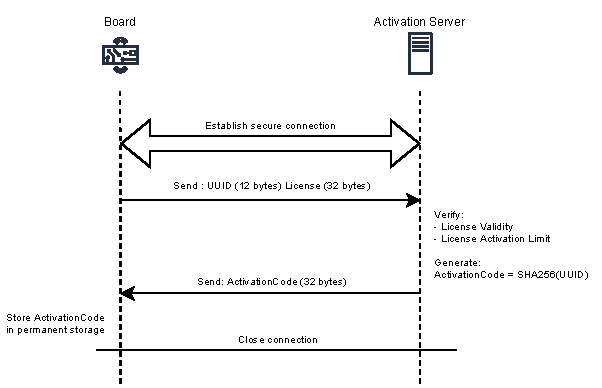
\includegraphics[scale=1.2]{images/activation.pdf}
	\caption{MCU-Fortifier activation process}
	\label{fig:activation}
\end{figure}

The microvisor checks for the device activation at every boot and launches the fortified application only if the board has been activated.
The activation process is normally performed on the first boot that has access to a valid internet connection. Figure \ref{fig:activation} highlights the different steps of the activation process:
\begin{enumerate}
	\item The microvisor opens a secure connection with the \textit{Activation Server}, a server controlled by Security Embedded used to activate new MCU-Fortifier installations.
	\item The microvisor sends the 32-byte license code and the 12-byte board UUID\footnote{Every STM board is provided with an immutable UUID useful for fingerprinting}. The license is specified by the user through the MCU-Fortifier configuration file.
	\item The Activation Server checks the validity of the license. The activation proceeds only if the license is valid and the number of activated devices has not been exceeded.
	\item The Activation Server generates a 32-byte \textit{activation code} by hashing the board UUID. The hash function used is \textit{sha256}. The activation code is then sent back to the board.
	\item The microvisor stores the newly received activation code in the permanent storage area described in Section \ref{subsec:permanent_storage}.
\end{enumerate}

Before launching the fortified application, the microvisor performs the activation check which consists in computing the expected activation codes and comparing it with the one received form the activation server (stored in permanent storage). If they match, the board is considered to be activated and the fortified application is launched, otherwise the board is restarted in an attempt to perform the activation process once more.

\subsubsection{Security Considerations}
The presented implementation does not provide a high degree of security against a malicious user aiming to use MCU-Fortifier without a valid license. In fact, it would be easy for such an user to inspect the activation check, using a debugger, and bypass it by generating the expected valid license.

Preventing the user form generating a valid license could be done trivially using asymmetric encryption. Encrypting the output of the \textit{sha256} function with the private key of the Activation Server would allow to obtain an activation code much harder to forge. The microvisor would then check the activation by decrypting it with the known public key and comparing the result with the expected hash.

This feature, however, was not implemented mainly for two reasons. Firstly, it does nor represent a ``real'' increase in security. In fact, without the use of other techniques (such as code obfuscation and other countermeasures) a malicious user could easily bypass the whole check altogether, removing the need to generate a valid activation code. Secondly, the development of MCU-Fortifier was already subjected to different delays, so the more simplistic approach was chosen.

\subsubsection{Activation Server}
MCU-Fortifier provides a Python 3 implementation of the Activation Server created as a way to demonstrate the licensing system of MCU-Fortifier in order to satisfy the development requirements. It's not meant to be used in a production environment as the valid licenses must be specified direcly in the source code. Additionally, the activation history for each license is only kept in volatile memory and lost upon reboot.

Nevertheless, it provides a valid starting point for the development of the production version. At the time of writing, it's not yet clear which platform/technologies will be used for the production version of the Activation Server. For example a NodeJS-based implementation combined with a web interface, could represent a valid option.

Regardless of the actual implementation, all the public-private key pairs and certificates provided are not meant to be used during production and should be regenerated.

\subsection{Remote Updates}
\label{subsec:OTA}
MCU-Fortifier provides the ability to perform update over-the-air (OTA). In particular both the on-board microvisor and the fortified application installed can be updated remotely although they follow slightly different procedures which will now be explained.
In both cases, the update process is performed by interacting with the \textit{Update Server} through a secure communication channel.

\subsubsection{Fortified Application Updates}
Updates to the fortified application are performed as following:
\begin{enumerate}
	\item The microvisor computes a checksum of the current fortified application, which is used as a fingerprint.
	\item The hash is sent to the Update Server asking for updates to the fortified application.
	\item The Update Server, who stores a table detailing which fortified application should be installed on the various boards, compares the hash received with the hash of the expected fortified application. If the hash matches, then the fortified application installed on the board is up to date. Otherwise the server notifies the microvisor that an update is available and prepares to transfer it.
	\item When an update is available, the microvisor deletes all the flash memory reserved to the fortified application, reads the size of the update and begins a downloading it in packets.
	\item After all packets have been downloaded and flashed, the checksum of the new fortified application is computed and sent to the server in order to verify that the update was successful.
\end{enumerate}

\paragraph{Checksum}
The checksum is performed using the hashing function \textit{sha256}. Additionally, the checksum covers all of the fortified application reserved flash memory in use. Meaning that empty flash memory, reserved for fortified application usage, is not covered by the checksum.

This is done in order to ease the computation of the hash on the Update Server side. In fact, the server only needs to hash the binary image of the update which is easily obtainable by passing the ELF executable to \textit{objcopy}.

On the other hand, if the checksum covered the entirety of the fortified application flash memory, the Update Server would need to pad the binary image with empty words (words with value \verb|0xffffffff| in case of our device) for the entire length of the reserved flash memory. This would be especially difficult since different devices might have different amounts of flash memory available and the server would need to know the exact amount bytes to pad (otherwise the checksum computed would be incorrect).

With our implementation instead, computing the hash on the server side is easy. The only downside being that the microvisor needs to store the size of the fortified application explicitly in order for the checksum to cover the correct amount of memory. This is done by using the permanent storage mechanism described in Section \ref{subsec:permanent_storage}. When performing an update, the size stored is updated as well in order to reflect the size of the newly installed fortified application.

Unfortunately the size of the fortified application is not always immediately available. This is normally the case when MCU-Fortifier and the fortified application are installed ``locally'' though the use of programmers or debugging interfaces (e.g. ST-Link). In this scenario the microvisor manually recomputes the correct firmware size by scrolling backwards the fortified application flash memory until the first non-empty word is found.
This approach is not always guaranteed to work. In fact, if the fortified flash memory was not completely cleared the microvisor could compute an incorrect size.

Fortunately, this represents a minor issue since the application would still work as normally. The only impacted component would be the checksum resulting, at worst, in a redundant update.

\paragraph{Update Splitting}
The microvisor downloads the update in chunks performing what we call a ``request-read-flash'' loop. This process consists in requesting a small chunk of the update to the server, reading its content and flashing it to the fortified application flash memory.

Transferring the update in small chunks is necessary because embedded devices generally lack the RAM needed to store it in its entirety and flash it in a single operation.

\subsubsection{Microvisor Updates}
Performing a microvisor update is more complex than performing a fortified application update. The reason being that the microvisor must update itself, meaning that the code in execution should delete itself from flash memory and write the new code.

Since this is not feasible the best alternative is to perform the update process in two steps: downloading the update and launching an in-RAM function to write it to flash memory.

Unfortunately, this process presents two main challenges:
\begin{itemize}
	\item Firstly, as previously mentioned, embedded devices do not have enough RAM to hold the whole update image.
	\item Secondly, an in-RAM function writing the update to flash memory is not ``self-contained'' meaning that it would perform calls to many other functions which would need to be stored in RAM as well.
\end{itemize}

\paragraph{Update Storage}
To solve the first problem we need a location to store the microvisor update before being flashed to its final location. For this reason, our implementation stores the update image received in the flash area dedicated to the fortified application.

This implies that a microvisor update erases the fortified application currently installed. In practice, this does not represent a problem since microvisor updates are rare and the fortified application can always be reinstalled after the update.

\paragraph{Update Install}
As already mentioned, we cannot use a ``self-contained'' in-RAM function to flash the update to the correct location. In fact, writing flash memory is a complex operation that requires interaction with peripherals (such as the flash controller) and specific timings (using system delays and tick counters).

In practice, instead of a single in-RAM function we need an entire in-RAM application. For our implementation we created a dedicated in-RAM application called \textit{reflasher}, because it reads the update image stored in the fortified application flash memory and writes it to its final destination, overwriting the previous version of the microvisor.

During normal operation however, the \textit{reflasher} utility is not stored in the microvisor flash memory as it would consume precious storage space. Instead, \textit{reflasher} is downloaded directly form the update server during the microvisor update process, meaning that it requires no additional storage space.

\paragraph{Update Steps}
To summarize, after the update server has confirmed that a microvisor update the following steps are performed:
\begin{enumerate}
	\item The fortified application flash memory is erased.
	\item The microvisor update is downloaded in packets and flashed to the fortified application flash memory.
	\item The \textit{reflasher} utility is downloaded and flashed immediately after the update image.
	\item Communication is over. The microvisor frees the RAM previously in use and copies the \textit{reflasher} utility to it.
	\item The microvisor begins executing \textit{reflasher} passing the required parameters (e.g. source and destination addresses of flash memory, amount of bytes to copy).
\end{enumerate}
At this point \textit{reflasher} begin its execution and performs the following:
\begin{enumerate}
	\item The microvisor reserved flash memory is erased.
	\item The microvisor update image is copied form the fortified application flash memory to the microvisor flash memory.
	\item The fortified application flash memory is erased. This step is required to ensure that neither the microvisor nor the \textit{reflasher} utility leak data that could be accesed by a fortified application installed in the future.
	\item The device is rebooted.
\end{enumerate}
After the reboot, if all the steps were executed succesfully, the updated microvisor begins its normal execution: checking the activation, contacting the update server, downloading a new fortified application and so on.

Unfortunately, errors might occur during the update process. For example, failing to write an address of flash memory. Most of these errors can be considered critical as there is no way to recover from them. This is especially true for any error that occurs during the execution of the \textit{reflasher} utility as the microvisor can be left in an unknown state.

In the worst scenario, the microvisor is corrupted and cannot be launched. This means that the board is ``bricked'' and a local update (using a programmer or debugging interfaces such as ST-Link) is required in order to reinstall MCU-Fortifier correctly.

This could represent a problems for board that are deployed on site and managed remotely. Fortunately, errors during flash programming are uncommon and have never occurred during our testing.

\paragraph{Microvisor Versioning}
Regarding microvisor updates, the checksum of the microvisor flash memory cannot be used as a way to compare the version installed with the update.

This problem arises due to the content stored in the \textit{permanent storage} (which is effectively a part of the microvisor flash memory) altering the result of the checksum unpredictably.

In the current implementation the microvisor accepts and installs any update provided by the server regardless of the version currently installed.
Nevertheless a versioning system could easily be integrated either by:
\begin{itemize}
	\item Separating the permanent storage from the microvisor flash memory and performing the checksum only on the latter one.
	\item Implementing a field indicating explicitly the version of the microvisor installed (e.g. a counter).
\end{itemize}
Due to time constraints during the development process we were not able to integrate one of these solution in the current version of MCU-Fortifier.

\subsubsection{Update Server}
\label{subsubsec:update_server}
Similarly to the Activation Server, the Update Server is also implemented as a Python 3 script in order to demonstrate the OTA update and error reporting capabilities provided by MCU-Fortifier.

As stated in the MCU-Fortifier User Manual\cite{user_manual}, the script can be modified in order to provide the pre-shared communication keys necessary for securing the communication with different devices. The user can provide binary images for updating both the fortified application and the microvisor in execution on devices. Additionally, during the boot the devices can also connect to the Update Server in order to report errors encountered at runtime.

Again, such implementation is not meant to be deployed in a production environment but rather used during development to showcase and test different functionalities. Similarly to the Activation Server, it can be used as a base for developing the production version of the Update Server.

\subsection{Error Reporting}
Among other features, MCU-Fortifier provides the ability to log errors and report them to the Update Server. Any error occurring during the execution of the microvisor or fortified application are logged in the permanent storage memory area. On subsequent boots, after the microvisor establishes a connection with the update server, the error is reported and deleted from permanent storage.

In the current implementation only a single error can be logged in permanent storage. This does not represent a limitation, since all the errors currently implemented are ``critical'' thus result in an immediate reboot of the device allowing to correctly report them.

In particular, the microvisor stores an \textit{Error ID} representing the error that occurred and some \textit{Error Data} containing additional information describing the error. Currently, the following errors are implemented:
\begin{itemize}
	\item Invalid License: triggered after attempting the activation process with an invalid MCU-Fortifier license.
	\item License Limit Exceeded: triggered after attempting the activation process with a license that has already exceeded the maximum number of allowed activation.
	\item MPU Error: triggered after a memory access that resulted in an MPU violation. The error data stores additional information about the access and is processed by the Update Server in order to provide a human-readable report.
\end{itemize}

\end{comment}

\begin{comment}
\newpage
\section{Repository Organization}
\label{sec:repo}
In this section we detail the structure of the MCU-Fortifier repository, the different folders and the macro-components implemented in each source file.

\subsection{Repository Root Directory}
\begin{figure}[h]
	\centering
	\begin{minipage}{7cm}
		\dirtree{%
			.1 MCU-Fortifier.
			.2 .vscode.
			.2 ActivationServer.
			.2 Documentation.
			.3 source\_manual.
			.3 user\_manual.
			.2 Drivers.
			.2 Microvisor.
			.3 Inc.
			.3 Private-Src.
			.3 Src.
			.2 Middlewares.
			.2 UpdateServer.
			.2 Utils.
			.2 .gitignore.
			.2 BOOTLOADER.ld.
			.2 Makefile.
			.2 memory\_map.ld.
			.2 startup\_bootloader.s.
		}
	\end{minipage}
\caption{Directory tree of MCU-Fortifier repository}
\label{fig:repo_tree}
\end{figure}

Figure \ref{fig:repo_tree} illustrates the content of the repository root directory. In particular, the following entries are present:
\begin{itemize}
	\item \verb|.vscode|: directory containing configuration files for VisualStudio Code IDE.
	\item \verb|ActivationServer|: directory containing all server side files regarding the Activation Server.
	\item \verb|Documentation|: directory containing both the MCU-Fortifier User Manual\cite{user_manual} and this manual.
	\item \verb|Drivers|: directory containing BSP, CMSIS and STM32L475 drivers.
	\item \verb|Microvisor|: directory containing Microvisor source code. \verb|Inc| folder contains all header files. \verb|Private-Src| contains source files not shared with MCU-Fortifier users. \verb|Src| contains publicly available source files.
	\item \verb|Middlewares|: directory containing third party libraries such as \textit{mbedtls} and the board Wi-Fi library.
	\item \verb|UpdateServer|: directory containing all server side files regarding the Update Server.
	\item \verb|Utils|: directory containing multiple utility scripts, including the instrumentation required to create fortified applications (\verb|instrumenter.py|).
	\item \verb|.gitignore|: git repository configuration file.
	\item \verb|BOOTLOADER.ld|: linker script used to build the MCU-Fortifier microvisor.
	\item \verb|Makefile|: Makefile automating the build process.
	\item \verb|memory_map.ld|: linker script containing the memory map.
	\item \verb|startup_bootloader.s|: assembly file including the entry point of MCU-Fortifier, the vector table used by the microvisor and the vector table used for the interrupt deprioritization mechanisms.
\end{itemize}

\paragraph{Private and Public Sources}
The division of sources between \verb|Private-Src| and \verb|Src| is done because MCU-Fortifier users must be able to modify some source files in order to specify more advanced configuration.

Of course we want to prevent end-users from having complete access over the entire source code. For this reason the \textit{Makefile} provides rules to compile and group all private sources together in order to create a library which is then used by end-users to generate their own customized version of MCU-Fortifier.

In the current implementation, the library generation process does not strip symbols form the generated object files for debugging purposes. In the future, it might be better to strip symbols in order to render more difficult any reverse engineering attempt on MCU-Fortifier.

\subsubsection{Microvisor Source Files and Macrocomponents}
We will now examine the different microvisor source files and the macrocomponents implemented by each of them:
\begin{itemize}
	\item \verb|activator|: implements MCU-Fortifier licensing system described in Section \ref{subsec:activation}.
	\item \verb|bootloader|: primary code unit of microvisor. Immediately called by \verb|Reset_Handler| after board reboot. Performs all necessary tasks (activation check, error reporting, update checking) before transitioning to fortified application execution.
	\item \verb|error|: contains different error codes and length of data associated with each error.
	\item \verb|exception_manager|: implements interrupt deprioritization routines described in Section \ref{subsec:deprio}.
	\item \verb|it|: implements microvisor system interrupts (handlers for \textit{HardFault}, \textit{SVCall} and \textit{MemManage} exceptions).
	\item \verb|mbedtls_rng_wrapper|: wrapper providing an interface between STM DRBG (Deterministic Random Bit Generator) peripheral and \textit{mbedtls} library.
	\item \verb|memory_map|: header file providing variables for memory map symbols defined in linker scripts.
	\item \verb|microvisor_config|: contains different configuration settings for the microvisor. Customized by the user before the compilation of MCU-Fortifier.
	
	The different configuration aspects are described in MCU-Fortifier User Manual\cite{user_manual}.
	\item \verb|ota|: implements OTA update capabilities for both microvisor and fortified applications. Described in Section \ref{subsec:OTA}.
	\item \verb|permanent_storage|: implements permanent storage system described in Section \ref{subsec:permanent_storage}.
	\item \verb|PPB_handlers|: implements simulation of different load/store encoding necessary to recover PPB accesses as described in Section \ref{subsubsec:PPB_access}.
	\item \verb|PPB_recovery|: implements instruction matching and correct handler selection for PPB access recovery. Described in Section \ref{subsubsec:PPB_access}.
	\item \verb|sec_comm|: implements secure communication layer used transparently by the rest of the system. Described in Section \ref{subsec:comm}.
	\item \verb|simulator_common|: simulation and utility functions used during PPB access recovery (Section \ref{subsubsec:PPB_access}) and system instruction simulation (Section \ref{subsubsec:system_instructions}).
	\item \verb|stm32l4xx_hal_conf|: import and configuration of HAL (Hardware Abstraction Layer) libraries provided by STMicroelectronics.
	\item \verb|stm32l4xx_hal_msp|: HAL MSP (MCU Support Package) callbacks. Used to configure clocks and other low-level properties of DRBG peripheral.
	\item \verb|stm32l4xx_it|: default system interrupts (provided by STM) used by microvisor before transitioning to fortified application execution and enforcing interrupt deprioritization.
	\item \verb|stm32l475vg_mpu|: MPU configuration for STM32L475 MCU. Described in Section \ref{subsec:MPU}.
	\item \verb|system_instruction_recovery|: system instruction recovery mechanisms described in Section \ref{subsubsec:system_instructions}.
	\item \verb|system_stm32l4xx|: system configuration of STM32L475 MCU. Provided by STMicroelectornics.
	\item \verb|virtual_IPSR|: implements virtual IPSR described in Section \ref{subsubsec:virtual_IPSR}.
	\item \verb|wifi_wrapper|: interface layer abstracting specific characteristics of the Wi-Fi peripheral equipped on our B-L475EIOT01A1 board. Used by the secure communication layer. Allows to easily port implementation to devices using different communication peripherals.
\end{itemize}

\end{comment}

\begin{comment}
\newpage
\section{Reflasher}
The \textit{reflasher} utility, being a complete separate application that runs in RAM, has a repository on its own.
In particular, the source code is available at:

\url{https://github.com/crosscon/baremetal-tee/tree/main/MPU-version/reflasher}
\end{comment}

%An additional repository containing different examples of instrumented applications, as well as the test cases used to demonstrate the capabilities of MCU-Fortifier and evaluate the development requirements is available at:

%\url{https://github.com/beaglehot/MCU-Fortifier-Examples}



% also  say that we can do local udpate (not only remote)?

% make it more similar to SuV? Talk about attackers model, which attacks can be prevented and such (e.g. no remote code executinon, code integrity (no write to flash) no overread to microvisor etc?)?

% maybe in design section add a subsection with capabiliteis of MCU fortifier? (given that flash is read only, code integrity is provided but not buffer overread on flash etc...)?


\clearpage
\bibliography{biblio}

\end{document}